\documentclass{beamer}
\usepackage{times}
\usepackage{tikz}
\usepackage{beamerthemesplit}
\usepackage{tcolorbox}
\usepackage{subfigure}

\title{A Tutorial of White-Box Cryptography \\ Chapter 5 Cryptanalysis}
\author{Zheng Gong\inst{1,2}\\ \url{cis.gong@gmail.com}}
\institute{\inst{1}{School of Computer Science, South China Normal University} \\ \inst{2}{Mobile Applications And Security Engineering Center of Guangdong Province}}

\date{\today}

\begin{document}

\frame
{
 \titlepage
}

\section[Outline]{}
\frame{\tableofcontents}

\section{Cryptanalysis of Chow \textit{et al.}'s White-box DES}
\frame
{
  \frametitle{Recall Chow et al.'s white-box DES}

\begin{itemize}
\item At ACM DRM 2002, Chow et al. proposed a white-box DES implementation for DRM applications.
\item The terminology and notation of this implementation are inherited in the following schemes.
\item In this very beginning paper of white-box cryptography, Chow \textit{et al.} use \textit{locally secure} to illustrate the protection of key extraction with the Man-At-The-End attack.
\end{itemize}

\begin{center}
\begin{tikzpicture}
    \node[anchor=south west,inner sep=0] (image) at (0,0) { 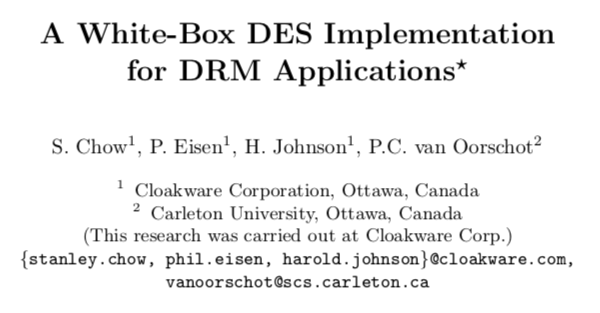
\includegraphics[width=7cm, height=3.5cm]{./pics/WBC_DES_2002.png}};

    %\begin{scope}[x={(image.south east)},y={(image.north west)}]
        %\draw[help lines,xstep=.1,ystep=.1] (0,0) grid (1,1);
        %\foreach \x in {0,1,...,9} { \node [anchor=north] at (\x/10,0) {0.\x}; }
        %\foreach \y in {0,1,...,9} { \node [anchor=east] at (0,\y/10) {0.\y}; }
        %\draw[green, ultra thick, rounded corners] (0.24,0.18) rectangle (0.50,0.32);
    %\end{scope}
\end{tikzpicture}
\end{center}
}

\subsection{Differential Fault Analysis of WBDES}

\frame
{
\frametitle{Differential fault analysis on the last round of the iterated block cipher}
On ACM DRM 2002, Jacob \textit{et al.} proposed a differential fault analysis on Chow \textit{et al.}'s white-box DES.
\begin{center}
\begin{tikzpicture}
    \node[anchor=south west,inner sep=0] (image) at (0,0) { 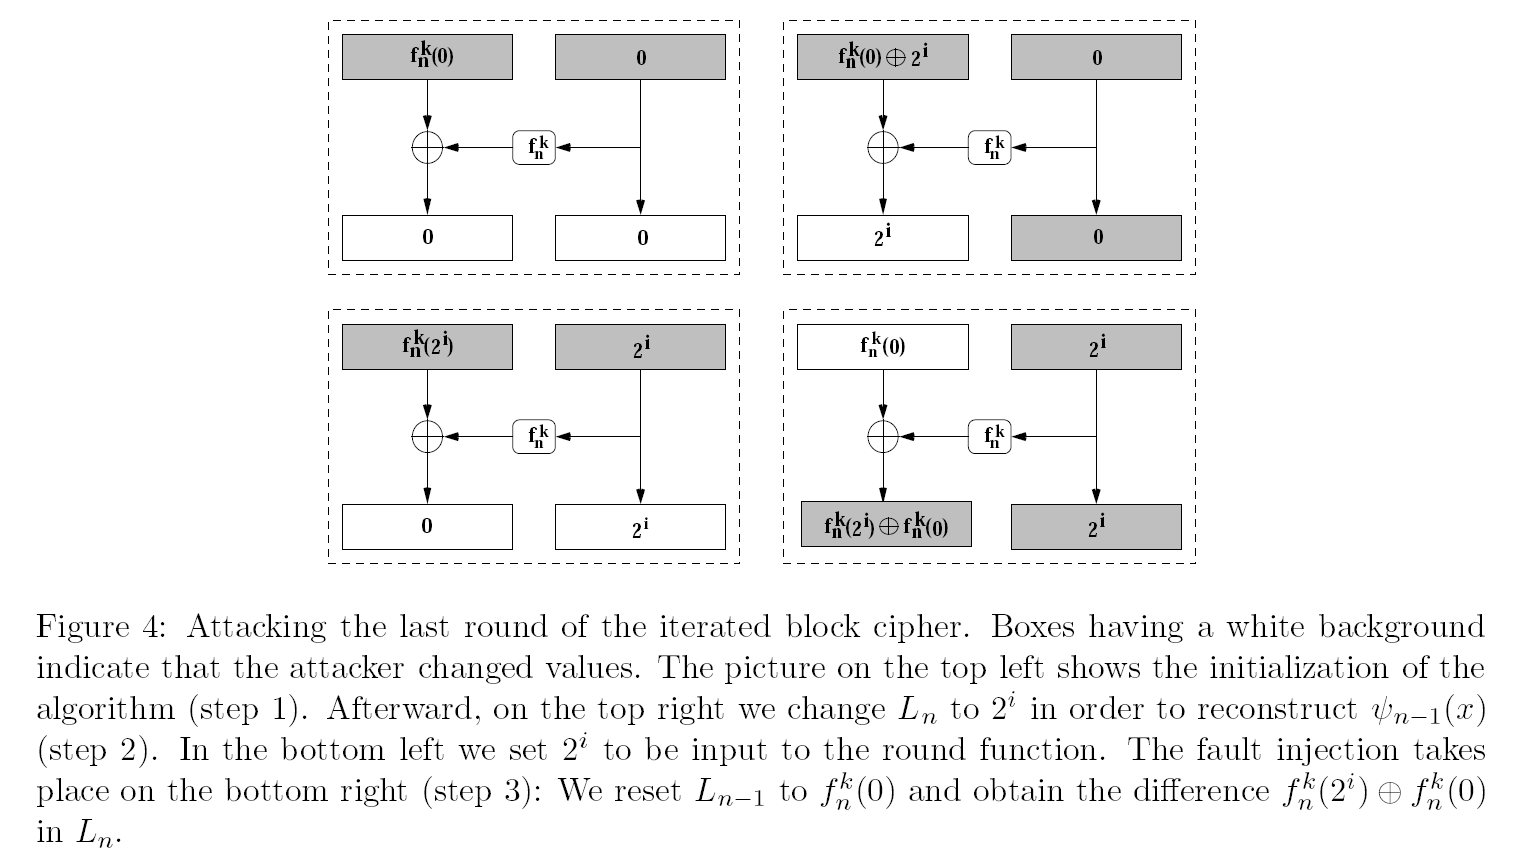
\includegraphics[width=10cm, height=5cm]{./pics/DFA_WBDES.png}};

    %\begin{scope}[x={(image.south east)},y={(image.north west)}]
        %\draw[help lines,xstep=.1,ystep=.1] (0,0) grid (1,1);
        %\foreach \x in {0,1,...,9} { \node [anchor=north] at (\x/10,0) {0.\x}; }
        %\foreach \y in {0,1,...,9} { \node [anchor=east] at (0,\y/10) {0.\y}; }
        %\draw[green, ultra thick, rounded corners] (0.24,0.18) rectangle (0.50,0.32);
    %\end{scope}
\end{tikzpicture}

\end{center}
}

\frame
{
\frametitle{The four steps of Jacob \textit{et al.}'s algorithm (1)}
\textbf{1. Initialization:}
\begin{enumerate}[1)]
\item Set $L_{n}=0$, $R_{n}=0$;
\item Compute $\theta_{n-1}(L_{n-1}, R_{n-1})=E^{k}_{n-1}(D^{k}(L_{n}, R_{n}))$;
\item Result: $L_{n-1}=f^{k}_{n}(0)$, $R_{n-1}=0$;
\item Derive $\Omega=\theta_{n-1}(L_{n-1}, R_{n-1})=\theta_{n-1}(f^{k}_{n}(0),0)$.
\end{enumerate}
}

\frame
{
\frametitle{The four steps of Jacob \textit{et al.}'s algorithm (2)}
\textbf{2. Reconstruct:}
\begin{enumerate}[(a)]
\item For $i=1$ to $m$:

\begin{enumerate}[1)]
\item Set $L_{n}=2^{i}$, $R_{n}=0$;
\item Compute $\theta_{n-1}(L_{n-1}, R_{n-1})=E^{k}_{n-1}(D^{k}(L_{n}, R_{n}))$;
\item Set $\Delta(i)=\theta_{n-1}(L_{n-1}, R_{n-1}) \oplus \Omega$;
\item For $j=1$ to $\frac{m}{4}$: If($\Delta(j) \neq 0$) $\rightarrow$ Set $\mathcal{O}(j)=\mathcal{O}(j) \cup {i}$;
\end{enumerate}

\item For $j=1$ to $m$:
\end{enumerate}
}

\frame
{
\begin{center}
\textbf{Thanks for your attentions!}
\end{center}
\begin{center}
\begin{tikzpicture}
    \node[anchor=south west,inner sep=0] (image) at (0,0) { 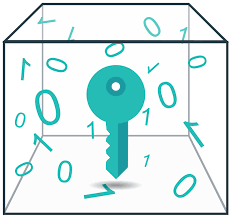
\includegraphics[width=4cm, height=4cm]{./pics/WBC_BG.png}};

    %\begin{scope}[x={(image.south east)},y={(image.north west)}]
        %\draw[help lines,xstep=.1,ystep=.1] (0,0) grid (1,1);
        %\foreach \x in {0,1,...,9} { \node [anchor=north] at (\x/10,0) {0.\x}; }
        %\foreach \y in {0,1,...,9} { \node [anchor=east] at (0,\y/10) {0.\y}; }
        %\draw[green, ultra thick, rounded corners] (0.24,0.18) rectangle (0.50,0.32);
    %\end{scope}
\end{tikzpicture}

\end{center}
}

\end{document}
